\documentclass[12pt,a4paper]{article}

% ============================================================
% PACKAGES
% ============================================================
\usepackage[
    a4paper,
    top=1.55cm,
    bottom=1.35cm,
    left=1.75cm,
    right=1.75cm
]{geometry}

\usepackage[T1]{fontenc}
\usepackage{newtxtext}
\usepackage{graphicx}
\usepackage{xcolor}
\usepackage{array}
\usepackage{tabularx}
\usepackage{fancyhdr}
\usepackage{tikz}
\usepackage{eso-pic}
\usepackage{ragged2e}

% ============================================================
% COLORS
% ============================================================
\definecolor{GEUBlue}{RGB}{43,91,145}
\definecolor{GEUBannerBlue}{RGB}{0,102,148}
\definecolor{GEUYellow}{RGB}{255,201,38}
\definecolor{InstructionGrey}{RGB}{125,125,125}

% ============================================================
% GENERAL SETTINGS
% ============================================================
\setlength{\parindent}{0pt}
\setlength{\parskip}{0pt}
\renewcommand{\arraystretch}{1}

% ============================================================
% HEADER / FOOTER
% ============================================================
\pagestyle{fancy}
\fancyhf{}

\fancyhead[L]{%
    \fontsize{10.5}{12}\selectfont
    Data Structure And Programming In C++ -- DSCPP
}

\fancyhead[R]{%
    \fontsize{10.5}{12}\selectfont
    PHASE-II PROJECT PROGRESS
}

\fancyfoot[R]{%
    \fontsize{10}{12}\selectfont
    Page \thepage
}

\renewcommand{\headrulewidth}{0pt}
\renewcommand{\footrulewidth}{0pt}

\setlength{\headheight}{20pt}
\setlength{\headsep}{0.65cm}
\setlength{\footskip}{0.65cm}

% ============================================================
% BOTTOM YELLOW LINE
% ============================================================
\AddToShipoutPictureBG{%
\begin{tikzpicture}[remember picture,overlay]
    \fill[GEUYellow]
    (current page.south west)
    rectangle
    ([yshift=0.14cm]current page.south east);
\end{tikzpicture}
}

% ============================================================
% CUSTOM COMMANDS
% ============================================================
\newcommand{\sectiontitle}[1]{%
    {\color{GEUBlue}
    \fontsize{18}{22}\selectfont #1}
}

\newcommand{\instruction}[1]{%
    {\color{InstructionGrey}
    \fontsize{10.5}{13}\selectfont #1}
}

\newcommand{\answerbox}[2]{%
    \begin{tabularx}{\textwidth}{
        |>{\RaggedRight\arraybackslash}X|}
        \hline
        \parbox[t][#1][t]{\dimexpr\linewidth-12pt\relax}{
            \vspace{5pt}
            \fontsize{11}{13}\selectfont #2
        }\\
        \hline
    \end{tabularx}
}

% ============================================================
% DOCUMENT
% ============================================================
\begin{document}

% ============================================================
% PAGE 1
% ============================================================

\vspace*{0.02cm}

% Logo + heading
\noindent
\begin{tabularx}{\textwidth}{@{}p{2.3cm}X@{}}

% Logo
\begin{minipage}[c][2.0cm][c]{2.3cm}
    \centering
    
\includegraphics[width=2.0cm]{logo.jpeg}
\end{minipage}
&
% Heading
\colorbox{GEUBannerBlue}{%
    \parbox[c][2.0cm][c]{\linewidth}{%
        \centering
        {\color{GEUYellow}
        \fontsize{16.5}{20}\selectfont
        \bfseries
        PROJECT AND TEAM INFORMATION}
    }
}

\end{tabularx}

\vspace{0.55cm}

% PROJECT TITLE
\sectiontitle{Project Title}

\vspace{0.05cm}

\vspace{0.40cm}

\answerbox{1.00cm}{RideSync: A Graph-Based Smart Cab Booking and Dispatch Simulation System}

\vspace{0.80cm}

% STUDENT INFORMATION
\sectiontitle{Student/Team Information}

\vspace{0.40cm}

\noindent
\begin{tabularx}{\textwidth}{
|>{\RaggedRight\arraybackslash}p{0.56\textwidth}
|>{\RaggedRight\arraybackslash}X|
}
\hline

\begin{minipage}[t]{\linewidth}
\vspace{1.5mm}
\textit{Team Name:}\\[-1mm]
\textit{Team ID:}
\vspace{1.5mm}
\end{minipage}
&
\begin{minipage}[t]{\linewidth}
\vspace{1.5mm}
\textit{The Four Bytes}\\[-1mm]
\textit{DSCPP-III-2026-T151}
\vspace{1.5mm}
\end{minipage}
\\
\hline

\begin{minipage}[t][3.25cm][t]{\linewidth}
\vspace{1.5mm}
\textbf{Team member 1 (Team Lead)}\\[-1mm]
\textit{(Last Name, name: student ID: email, picture):}
\vspace{2.0cm}
\end{minipage}
&
\begin{minipage}[t][3.25cm][t]{\linewidth}
\vspace{1.5mm}
\footnotesize
\textit{Gupta, Tanvi -- 2510010362}\\
\textit{tanvigupta2005.tg@gmail.com}

\vspace{2mm}
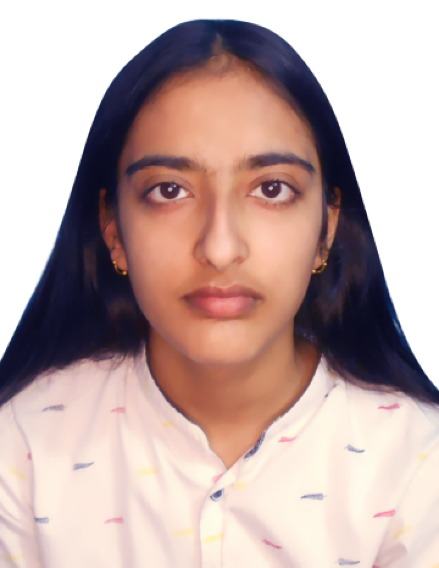
\includegraphics[width=3.0cm,height=1.5cm,keepaspectratio]{t.jpeg}
\end{minipage}
\\
\hline

\begin{minipage}[t][3.25cm][t]{\linewidth}
\vspace{1.5mm}
\textbf{Team member 2}\\[-1mm]
\textit{(Last Name, name: student ID: email, picture):}
\vspace{2.0cm}
\end{minipage}
&
\begin{minipage}[t][3.25cm][t]{\linewidth}
\vspace{1.5mm}
\footnotesize
\textit{Jahnavi -- 2510380066}\\
\textit{jahnavimittal89@gmail.com}

\vspace{2mm}
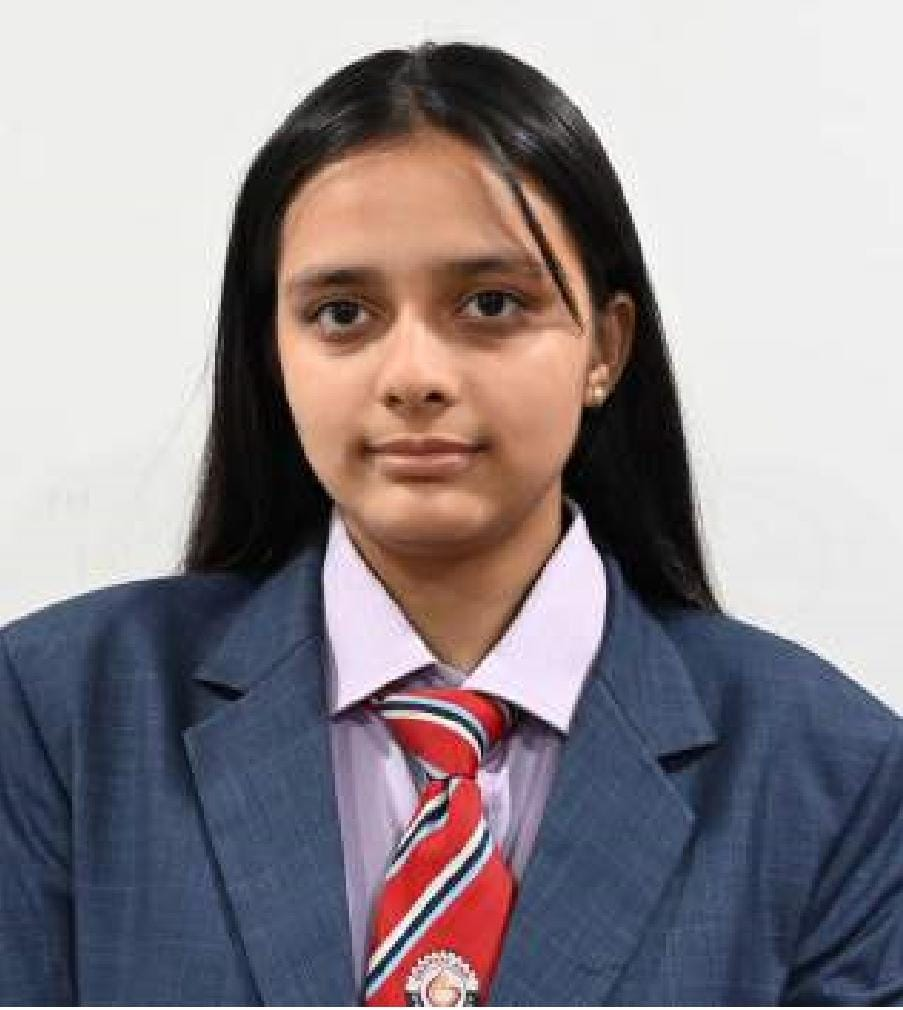
\includegraphics[width=3.0cm,height=1.5cm,keepaspectratio]{j.jpeg}
\end{minipage}
\\
\hline

\begin{minipage}[t][3.25cm][t]{\linewidth}
\vspace{1.5mm}
\textbf{Team member 3}\\[-1mm]
\textit{(Last Name, name: student ID: email, picture):}
\vspace{2.0cm}
\end{minipage}
&
\begin{minipage}[t][3.25cm][t]{\linewidth}
\vspace{1.5mm}
\footnotesize
\textit{Tyagi, Nishtha -- 2510370096}\\
\textit{nishthatyagii29@gmail.com}

\vspace{2mm}
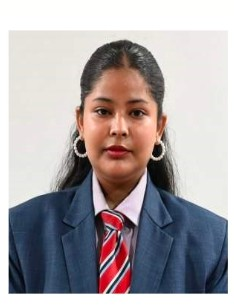
\includegraphics[width=3.0cm,height=1.5cm,keepaspectratio]{n .jpeg}
\end{minipage}
\\
\hline

\begin{minipage}[t][3.25cm][t]{\linewidth}
\vspace{1.5mm}
\textbf{Team member 4}\\[-1mm]
\textit{(Last Name, name: student ID: email, picture):}
\vspace{2.0cm}
\end{minipage}
&
\begin{minipage}[t][3.25cm][t]{\linewidth}
\vspace{1.5mm}
\footnotesize
\textit{Sharma, Dhairya -- 2510011490}\\
\textit{sharmadhairya820@gmail.com}

\vspace{2mm}
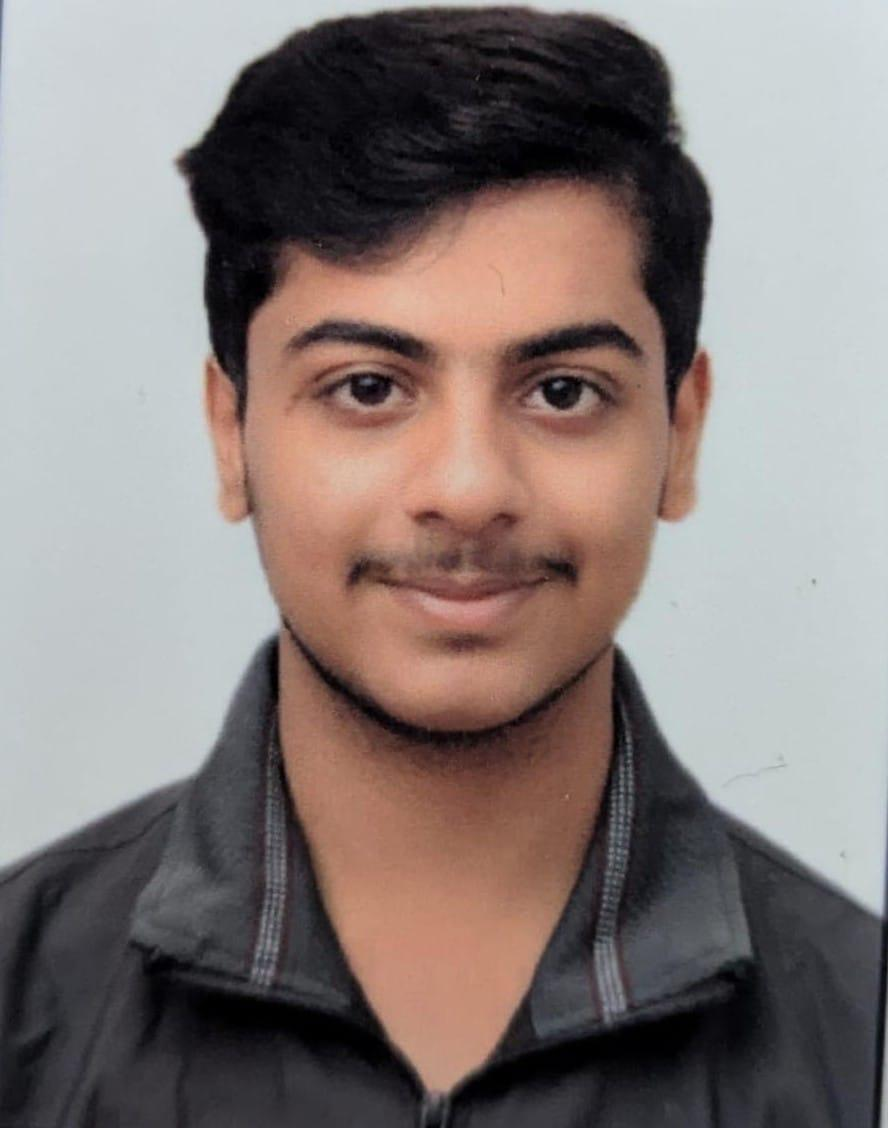
\includegraphics[width=3.0cm,height=1.5cm,keepaspectratio]{d.jpeg}
\end{minipage}
\\
\hline

\end{tabularx}

\vspace{0.45cm}

% ============================================================
% MENTOR INFORMATION
% ============================================================
\noindent
\begin{tabularx}{\textwidth}{
|>{\RaggedRight\arraybackslash}p{0.56\textwidth}
|>{\RaggedRight\arraybackslash}X|
}
\hline

\begin{minipage}[t]{\linewidth}
\vspace{2mm}
\textbf{Mentor Name:}\\[-1mm]
\textbf{Mentor Email Address:}
\vspace{2mm}
\end{minipage}
&
\begin{minipage}[t]{\linewidth}
\vspace{2mm}
\textit{Dr. Hemant Singh Pokhariya}\\
\textit{hemantsinghpokhariya@geu.ac.in}
\vspace{2mm}
\end{minipage}
\\
\hline

\end{tabularx}

\newpage

% ============================================================
% PAGE 2
% ============================================================

\vspace*{0.15cm}

\noindent
\colorbox{GEUBannerBlue}{%
\parbox{\dimexpr\textwidth-2\fboxsep\relax}{
    \vspace{0.18cm}
    {\color{GEUYellow}
    \fontsize{17}{21}\selectfont
    \bfseries
    PHASE-II PROJECT PROGRESS DESCRIPTION}
    \vspace{0.18cm}
}}

\vspace{0.70cm}

% PROJECT ABSTRACT
\sectiontitle{Project Abstract}

\vspace{0.05cm}

\vspace{0.12cm}

\answerbox{4.60cm}{
The main goal of our project, RideSync, is to build a console-based Cab Booking System in C++17. Booking a cab by phone call or at a taxi stand is unorganised. Customers cannot easily find the nearest cab, drivers are assigned manually without checking distance or availability, and there is no proper way to find the shortest path between the pickup and drop locations.

In this project customers, drivers and cabs are being handled through Object oriented programming. City locations and roads are stored as weighted graphs and shortest route calculation is done through Dijkstra's Algorithm. Driver assignment is done using a priority queue. Fare is then calculated from route ditance and the data is saved in these files so that it can be stored between runs. Our project does not use GPS, instead uses predefined locations.
}

\vspace{0.70cm}

% UPDATED PROJECT APPROACH
\sectiontitle{Updated Project Approach and Architecture}

\vspace{0.05cm}

\vspace{0.25cm}

\answerbox{7.60cm}{
Our implementation is based on C++17 and basic OOP principles. We have divided the system into the classes Customer, Driver, Cab, Admin and Booking. Their data members are private and are accessed through public functions. An Authentication Manager handles user login, and the Booking Manager works as the main controller that connects routing, fare calculation and driver assignment.

The city map is stored as an adjacency list using \texttt{std::unordered\_map<int, std::vector<std::pair<int, int>{}>{}>}. The shortest path and distance between pickup and drop locations are found using Dijkstra's Algorithm with \texttt{std::priority\_queue}. A second priority queue ranks the nearby available drivers using a score made from distance and rating, so the best driver can be assigned.

We use STL containers (vector, queue, priority queue, unordered map, and a stack for recent booking history) instead of writing our own, so that we can focus on the main logic. User and booking records are saved in flat text files between runs. Each module has its own header and source file. We have also added input validation for things like wrong location IDs or out-of-service cabs, so that the program does not crash.

The system is console-based, so no network communication protocol is used. All four members work together using GitHub and VS Code, and each module is unit tested before integration.
}

\newpage

% ============================================================
% PAGE 3
% ============================================================
\vspace*{0.20cm}

% TASKS COMPLETED
\sectiontitle{Tasks Completed}

\vspace{0.05cm}

\vspace{0.20cm}

\begin{tabularx}{\textwidth}{
|>{\RaggedRight\arraybackslash}X
|>{\RaggedRight\arraybackslash}p{0.28\textwidth}|
}
\hline

\textbf{Task Completed} &
\textbf{Team Member}\\
\hline

Problem definition, requirement analysis and overall system design (Phase 1) &
All team members \\
\hline

Design of the object-oriented class structure (Customer, Driver, Cab, Admin, User, and AuthManager) &
Tanvi Gupta \& Nishtha Tyagi \\
\hline

Implementation of User authentication, credential validation, and role management &
Tanvi Gupta \& Nishtha Tyagi \\
\hline

Initial architectural design and framework for the City Graph and Dijkstra route engine &
Jahnavi \\
\hline

Initial design and priority queue data structure formulation for Driver Dispatch &
Dhairya Sharma \\
\hline

\end{tabularx}

\vspace{0.65cm}

% CHALLENGES
\sectiontitle{Challenges/Roadblocks}

\vspace{0.05cm}

\vspace{0.18cm}

\answerbox{5.30cm}{
1. Dividing the work equally among four members and joining separate modules via GitHub commits. We have structured the code into distinct header and source files to ensure clean individual contributions.

2. Handling wrong inputs such as invalid location IDs or out-of-service cabs, which can crash the console program. We are adding robust input validation to each module.

3. Deciding how to combine distance and driver rating into one score for the driver priority queue. We tested composite score weightings to ensure optimal dispatching.

4. Making sure every module works properly before integration. We unit tested each component individually before building the central integration workflow.
}

\vspace{0.65cm}

% TASKS PENDING
\sectiontitle{Tasks Pending}

\vspace{0.05cm}

\vspace{0.18cm}

\begin{tabularx}{\textwidth}{
|>{\RaggedRight\arraybackslash}X
|>{\RaggedRight\arraybackslash}p{0.34\textwidth}|
}
\hline

\textbf{Task Pending} &
\textbf{Team Member (to complete the task)} \\
\hline

Graph representation of city locations using adjacency list map &
Jahnavi \\
\hline

Dijkstra's Algorithm implementation for shortest path routing &
Jahnavi \\
\hline

Priority-queue-based driver assignment using composite score &
Dhairya Sharma \\
\hline

Booking system logic and dynamic distance-based fare calculation &
Tanvi Gupta \& Nishtha Tyagi \\
\hline

File handling (`fstream`) persistence for booking history and trip logs &
Tanvi Gupta \& Nishtha Tyagi \\
\hline

System integration, end-to-end testing, and final demonstration &
All team members \\
\hline

\end{tabularx}

\newpage
% ============================================================
% PAGE 4
% ============================================================

\vspace*{0.30cm}

% PROJECT OUTCOME
\sectiontitle{Project Outcome/Deliverables}

\vspace{0.05cm}

\vspace{0.35cm}

\answerbox{7.7cm}{
By the end of the project, we expect to deliver a working console-based Cab Booking System in C++17 with the following parts:

\begin{itemize}
\setlength{\itemsep}{0pt}
\setlength{\topsep}{2pt}
\item Customer module: registration, login, cab booking and booking history
\item Driver module: registration, login and availability management
\item Admin module: managing cabs and drivers and viewing basic statistics
\item Route module: shortest path between pickup and destination using Dijkstra's Algorithm
\item Driver assignment using a priority queue
\item Fare calculation based on route distance
\item File-based storage for customer, driver, cab and booking data
\item Booking history and cancellation handling for customers
\item A short project report with basic testing documentation
\item A GitHub repository with the complete source code and commit history
\end{itemize}
}

\vspace{0.75cm}

% PROGRESS OVERVIEW
\sectiontitle{Progress Overview}

\vspace{0.05cm}

\vspace{0.25cm}

\answerbox{5.00cm}{


Phase 1: Problem definition, requirement analysis and system design is completed.

Phase 2: Class structure, authentication manager and basic Customer, Driver and Admin modules have also been worked on as planned.

Phase 3: The main algorithmic components, which are the location graph, Dijkstra's Algorithm and the priority queue for driver assignment, are still pending.

Phase 4: The booking system, fare calculation and file handling will be completed in Weeks 7 to 8.

Phase 5: Integration, testing and documentation are planned for Weeks 9 to 10.

Right now we are following our planned schedule, and no part is ahead of schedule.

}

\newpage

% ============================================================
% PAGE 5
% ============================================================

\vspace*{0.20cm}

% CODEBASE
% ---------- Codebase Information ----------
\vspace*{0.20cm}
\sectiontitle{Codebase Information}
\vspace{0.05cm}
\vspace{0.20cm}

\answerbox{9.0cm}{
\textbf{Repository link:} \texttt{github.com/TanviGupta12/RideSync-Cab-Booking-Dispatch}\\[3pt]
\textbf{Branch:} main\\[5pt]

Our team uses GitHub for sharing and managing the code, and VS Code for development. Every module is kept in its own header and source file, and the commit history shows the contribution of each team member.\\[5pt]

\textbf{Important Commits}
\vspace{-3pt}

\begin{itemize}
    \setlength{\itemsep}{2pt}
    \setlength{\parskip}{0pt}
    \setlength{\topsep}{2pt}
    \setlength{\leftmargin}{15pt}
    \small

    \item \textbf{Tanvi Gupta:} Initialized README, project structure, and base User class architecture.

    \item \textbf{Jahnavi:} Implemented CityGraph adjacency list and Dijkstra's shortest-path routing algorithm.

    \item \textbf{Nishtha Tyagi:} Developed derived Customer and Driver classes with rating and location tracking.

    \item \textbf{Dhairya Sharma:} Created the DriverMatchScore structure and priority-queue max-heap dispatch logic.

    \item \textbf{Tanvi Gupta:} Implemented dynamic distance-based fare calculation and file logging using fstream.

    \item \textbf{Dhairya Sharma:} Integrated priority-queue driver matching with shortest-path calculations.

    \item \textbf{Nishtha Tyagi:} Added std::stack-based storage for retrieving customers' recent booking history.

    \item \textbf{Tanvi Gupta:} Finalized CLI integration and connected the modular components in main.cpp.
\end{itemize}
}

\vspace{0.35cm}


% TESTING
\sectiontitle{Testing and Validation Status}

\vspace{0.05cm}
\vspace{0.30cm}


\begin{tabularx}{\textwidth}{
|>{\RaggedRight\arraybackslash}p{0.30\textwidth}
|>{\RaggedRight\arraybackslash}p{0.22\textwidth}
|>{\RaggedRight\arraybackslash}X|
}
\hline

\textbf{Test Type} &
\textbf{Status (Pass/Fail)} &
\textbf{Notes}
\\
\hline

Unit testing of each module
&
In progress
&
Each module is tested before integration. Results for the basic modules will be updated.
\\
\hline

Input validation testing
&
Pending
&
Wrong location IDs and out-of-service cabs will be checked.
\\
\hline

Integration testing
&
Pending
&
Planned in Phase 5 after all modules are ready.
\\
\hline

\end{tabularx}

\vspace{0.65cm}

% DELIVERABLES PROGRESS
\sectiontitle{Deliverables Progress}

\vspace{0.05cm}

\vspace{0.25cm}

\answerbox{6.20cm}{
Customer, Driver and Admin modules: In progress (basic versions)\\[2pt]
Route module (Dijkstra's Algorithm): Pending\\[2pt]
Priority-queue-based driver assignment: Pending\\[2pt]
Fare calculation: Pending\\[2pt]
File-based storage: Pending\\[2pt]
Booking history and cancellation handling: Pending\\[2pt]
Project report and testing documentation: Pending\\[2pt]
GitHub repository: In progress
}

\end{document}
